%%%%%%%%%%%%%%%%%%%%%%%%%%%%%%%%%%%%%%%%%%%%%%%%%%%%%%%%%%%%%%%%%%%%%%%%%%%%%%%%
%2345678901234567890123456789012345678901234567890123456789012345678901234567890
%        1         2         3         4         5         6         7         8

\documentclass[letterpaper, 10 pt, conference]{ieeeconf}  % Comment this line out if you need a4paper
%\documentclass[a4paper, 10pt, conference]{ieeeconf}      % Use this line for a4 paper

\IEEEoverridecommandlockouts                              % This command is only needed if 
                                                          % you want to use the \thanks command
\overrideIEEEmargins                                      % Needed to meet printer requirements.

% See the \addtolength command later in the file to balance the column lengths
% on the last page of the document

% The following packages can be found on http:\\www.ctan.org
\usepackage{graphicx} % for pdf, bitmapped graphics files
%\usepackage{epsfig} % for postscript graphics files
%\usepackage{mathptmx} % assumes new font selection scheme installed
%\usepackage{times} % assumes new font selection scheme installed
%\usepackage{amsmath} % assumes amsmath package installed
\usepackage{amssymb}  % assumes amsmath package installed

\title{\LARGE \bf
Dynamic Analysis of Sit-to-Stand Motion using Reachable Sets
}


\author{Sarah Seko, Sylvia Herbert, Robert Peter Matthew, Ruzena Bajcsy, Claire J. Tomlin% <-this % stops a space
%\thanks{*This work was not supported by any organization}% <-this % stops a space
\thanks{S. Seko, S. Herbert, R.P. Matthew, R. Bajcsy, and C. Tomlin  are with the Department of Electrical Engineering and Computer Science,
        University of California at Berkeley, Berkeley, CA, 94720,
        {\tt\small \{seko, sylvia.herbert, rpmatthew, bajcsy, tomlin\}@eecs.berkeley.edu}}%
}

\begin{document}

\maketitle
\thispagestyle{empty}
\pagestyle{empty}


%%%%%%%%%%%%%%%%%%%%%%%%%%%%%%%%%%%%%%%%%%%%%%%%%%%%%%%%%%%%%%%%%%%%%%%%%%%%%%%%
\begin{abstract}

The sit-to-stand (STS) motion is an essential activity of daily living and commonly used clinical assessment. In this paper, we introduce a method for the quantitative analysis of STS capability using Hamilton-Jacobi reachability. This approach computes the backwards reachable set, defined as the set of states from which standing is achievable. We model STS as a hybrid system with two modes representing the seated and rising phases of the action. The framework considers the dynamics and constraints of each mode and accounts for the seat-off transition. We present preliminary results for typical and limited joint torque capabilities...results?... This serves as a proof of concept for applying reachable set tools to the analysis of STS dynamics. 

\end{abstract}

%%%%%%%%%%%%%%%%%%%%%%%%%%%%%%%%%%%%%%%%%%%%%%%%%%%%%%%%%%%%%%%%%%%%%%%%%%%%%%%%

\section{INTRODUCTION}

Standing from a seated position is a common, yet biomechanically demanding action. The STS motion requires large joint torques and range of motion in comparison to other lower body functional tasks\cite{riley1991}. As a result, the elderly and those with limited motor function can experience difficulty when performing STS \cite{hughes1996}. Variations in STS have been studied in specific subject populations such as knee arthroplasty \cite{su1998} and Parkinson's disease \cite{Mak2013} patients. In a clinical setting, STS is used as a measure of mobility, motor function, and risk of falling \cite{whitney2005}, \cite{campbell1989}. However, clinical assessments are qualitative or imprecise, relying on measures such and five-times STS test \cite{whitney2005} or the timed-up-and-go test \cite{podsiadlo1991}.

While the kinematics of STS have been extensively studied, it remains challenging to quantify the dynamic stability. Existing methods have considered the velocity and acceleration of whole-body center of mass (COM) \cite{fujimoto2012} to compute the basin of stability. This paper presents a method for the quantitative analysis of STS dynamics using reachable sets. Hamilton-Jacobi reachability analysis provides a tool for the analysis of safety guarantees in controlled dynamical systems. This method allows for the computation of reachable sets, defined as the set of states from which a defined target set of states can be reachable. These methods have been applied to robotics and autonomous vehicle applications...tools for numerical computation of reachable set exist \cite{mitchell2004}. Dimensionality issues...?

This method can be applied as a metric for STS capability and used to analyze how an individual's deficiencies may impact their STS ability. Additionally, it can provide insight for healthcare providers in how to direct an individual to safely perform the motion. Finally, the method may be used as reference for guiding the design and controller-synthesis of devices aimed at assisting the STS motion.

We first formalize a hybrid system dynamic model of STS, representing the sitting and rising phases. For each mode, we present a rigid-body link model, and define kinematic and dynamic constraints on the system. We then use reachability analysis to compute the backwards reachable set of standing. We apply these methods to a human with typical and reduced joint torque capabilities....demonstrating the potential for this method to be used in further analysis of STS. Preliminary validation is performed through comparing data from a single subject performing three STS methods. 



\section{Sit-to-stand Model}

\subsection{Two-Mode Hybrid Model}

The STS motion has been described as a series of phases \cite{etnyre2007}, \cite{schenkman1990}, based on observed kinematic characteristics. From a dynamic systems perspective, the action can be divided into two discrete modes: a sitting phase and a rising phase. The system dynamics switch when contact with the chair is lost. At this instant, denoted seat-off, the human transitions from a stable system to a potentially unstable system \cite{etnyre2007}. Once seat-off occurs, the system remains within the rising mode dynamics as long as the sole point of external contact is between the feet and ground. While previous work has classified STS into three or four phases, this two-mode model incorporates the only change in dynamics without further constraining the action. The hybrid and biomechanical models are show in Figure \ref{fig: dynamics}.

\subsection{Dynamical Model}

We consider a rigid-body model of the human constrained to the sagittal plane. This model consists of three segments: shank, thigh, and HAT (head-arms-trunk), with corresponding joints: ankles, knees, and hips \cite{music2008}, \cite{matthew2016}. The nonlinear dynamics of the system are represented by

\begin{equation}
\dot{x}=f(x,u) 
\end{equation}
where the states $x= \left[\theta_a, \dot{\theta_a}, \theta_k, \dot{\theta_k},\theta_h,\dot{\theta_h}, \right] \in \mathbb{R}^6$ correspond to the ankle, knee, and hip angles and angular velocities, and the inputs $u = \left[\tau_a, \tau_k, \tau_h, \right] \in \mathbb{R}^3$ correspond to the joint torques.

The equations of motion,  derived through Lagrangian dynamics, and are described by:

\begin{equation}
M\left(\theta\right)\ddot{\theta} + C(\theta, \dot{\theta})\dot{\theta} + N \left(\theta\right) = \tau
\end{equation}

where $M$ represents the inertial forces due to acceleration of the joints, $C$ represents the Coriolis and centrifugal forces, $N$ represents the potential matrix, and $\tau$ is the applied joint torques. Model parameters such as lengths, masses, COM, and COM locations along segments were selected from literature values \cite{plagenhoef1983}. 


\begin{figure}[h]
  \centering
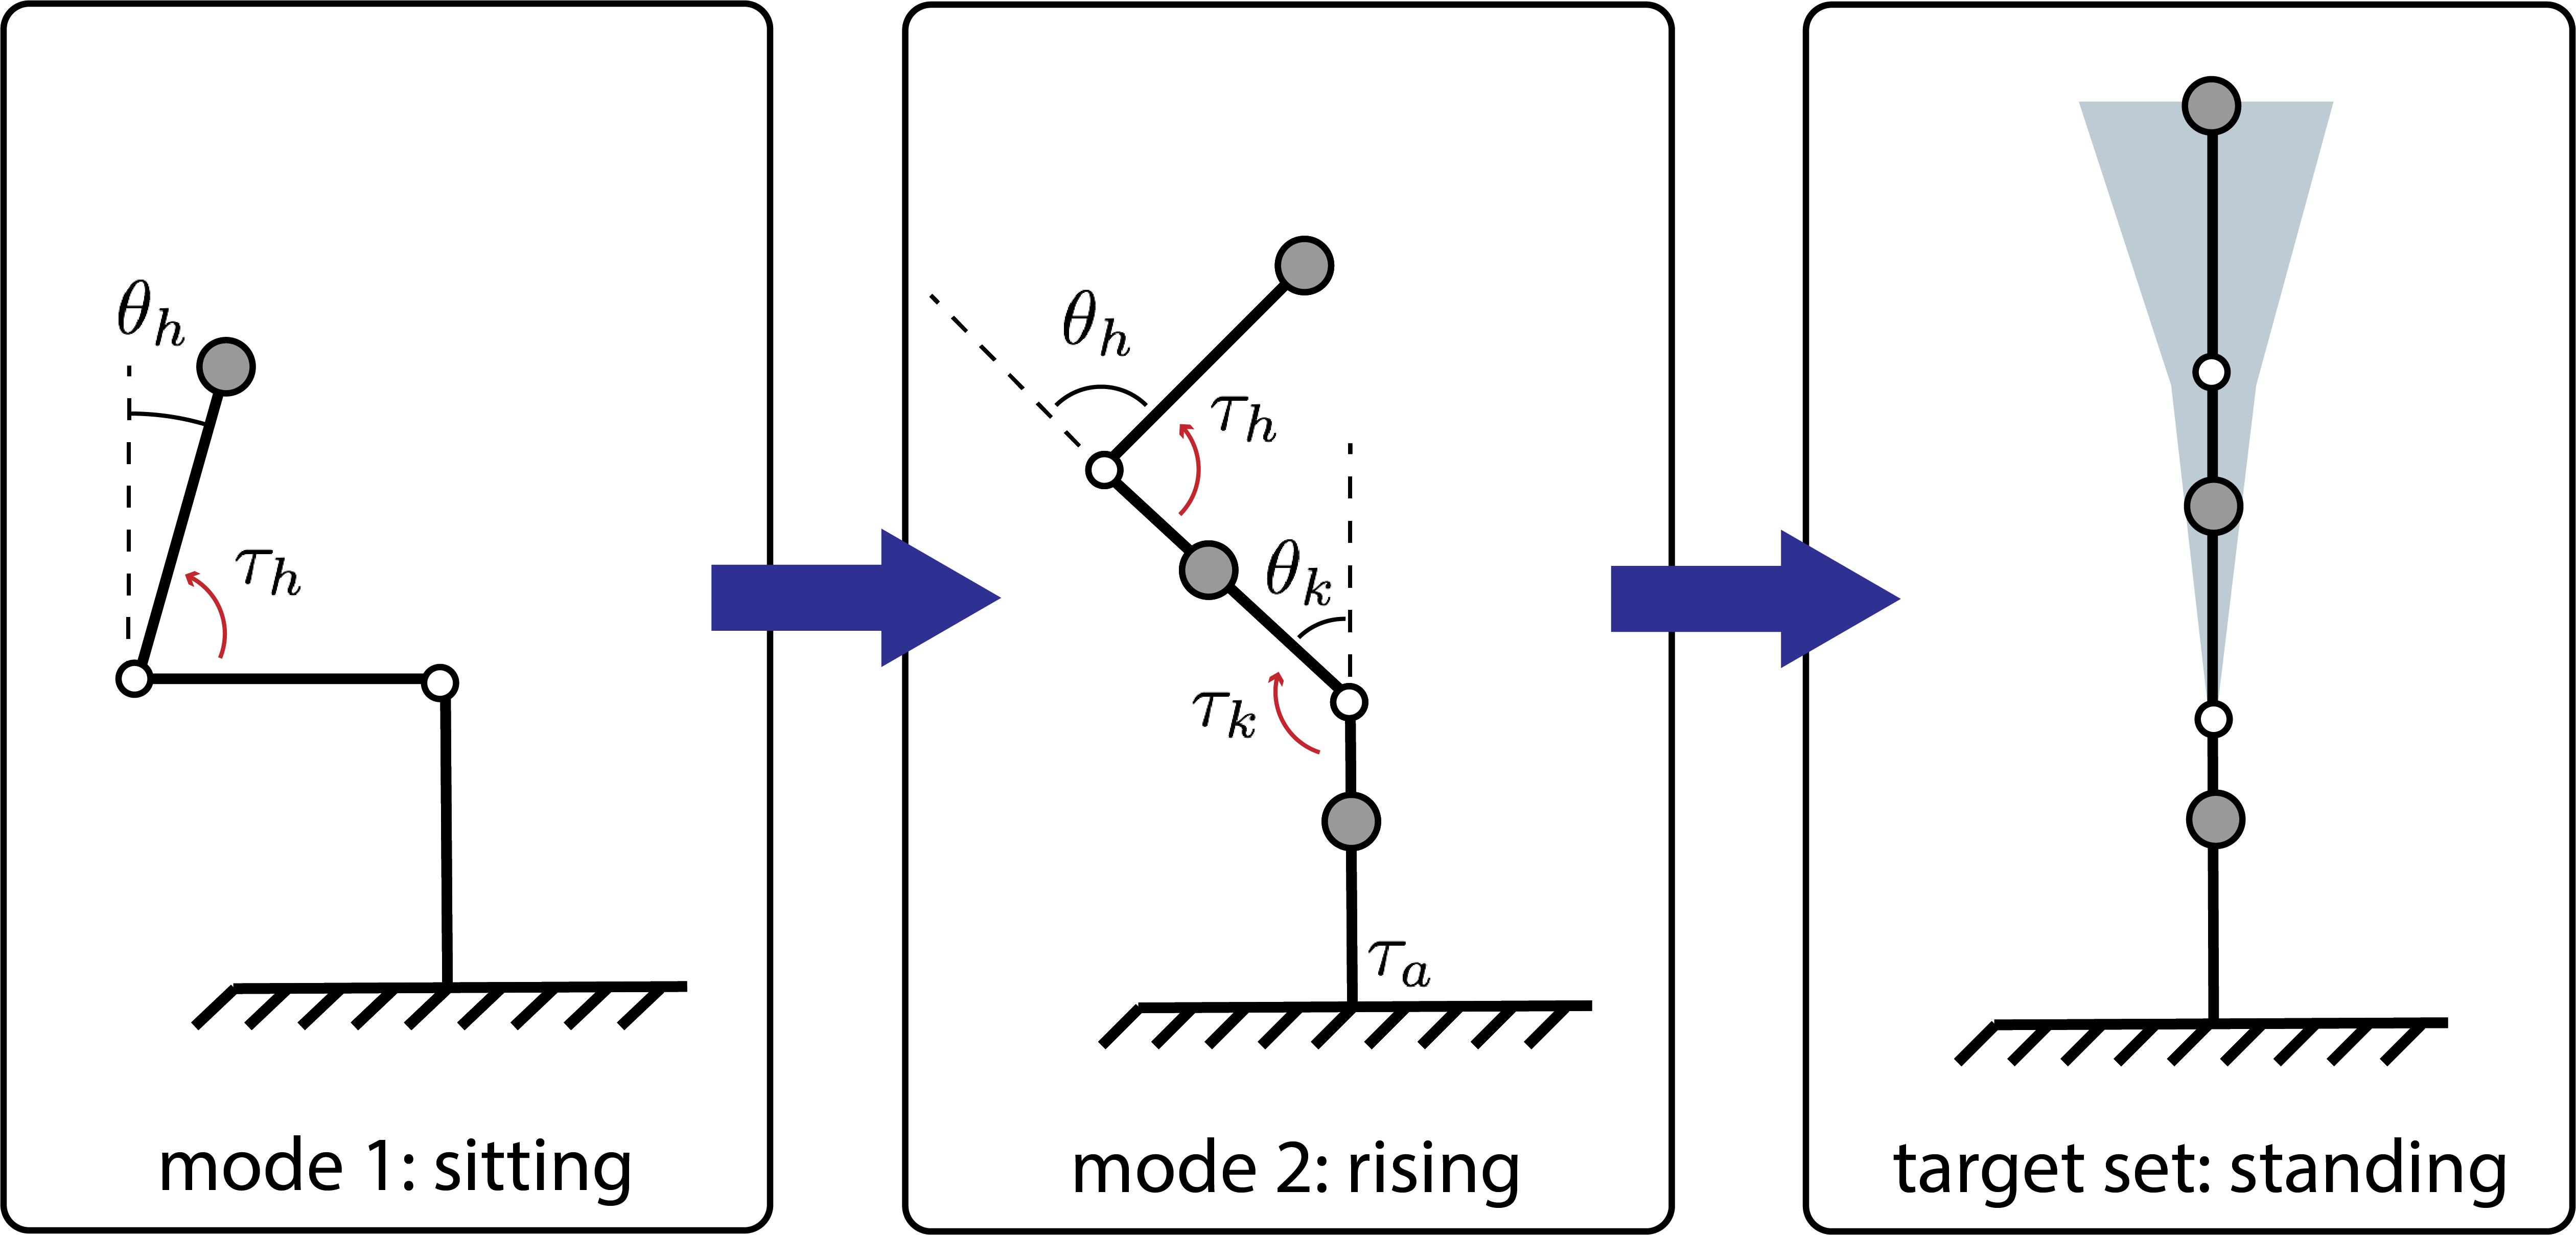
\includegraphics[width=3.4in]{figures/hybridSys.png}
\caption{Hybrid and biomechanical model of STS motion.}
  \label{fig: dynamics}
\end{figure}

Due to the computational complexity of reachability for a 6-D system, we propose a simplified model of the three segment body. During the sit-to-stand motion, the knee and hip joints exhibit greater variation in joint angle and angular velocity than the ankle joint. Thus, for initial investigation of this method, we assume the shank remains at a fixed position throughout the motion. The simplified model consists of a double inverted pendulum attached to a fixed link. Despite the limited range of motion of the ankle during STS, the joint experiences a large torque from the motion of the other body segments. We compute the resultant torque on the ankle and incorporate maximum bounds on the ankle torque when computing reachable sets. 

Alternative lower dimensional models of STS, including a telescopic pendulum\cite{papa1999} and double pendulum \cite{roberts1996} models, have been studied. However, a three-link model was selected due to its resemblance to human morphology and the direct correspondence between system inputs and joint torques. 

The above model is not representative of the seated phase due to the contact between the hips and the chair. During this phase the human bends the torso at the hip, generating momentum before leaving the seat. We model this phase as a single inverted pendulum anchored at the hip joint with the segment representing the HAT. These simplified dynamics are described by:

\begin{equation}
\ddot{\theta_h} = \frac{g}{l} \sin{\theta_h} + \frac{1}{ml^2} \tau_h
\end{equation}

%\subsection{Kinematic and Joint Torque Constraints}

Kinematic constraints on the joint angle range of motion and maximum angular velocities are set. A constraint on the maximum voluntary joint torque was placed on each joint. 

\section{Reachable Set Analysis}

\begin{figure}
	\centering
	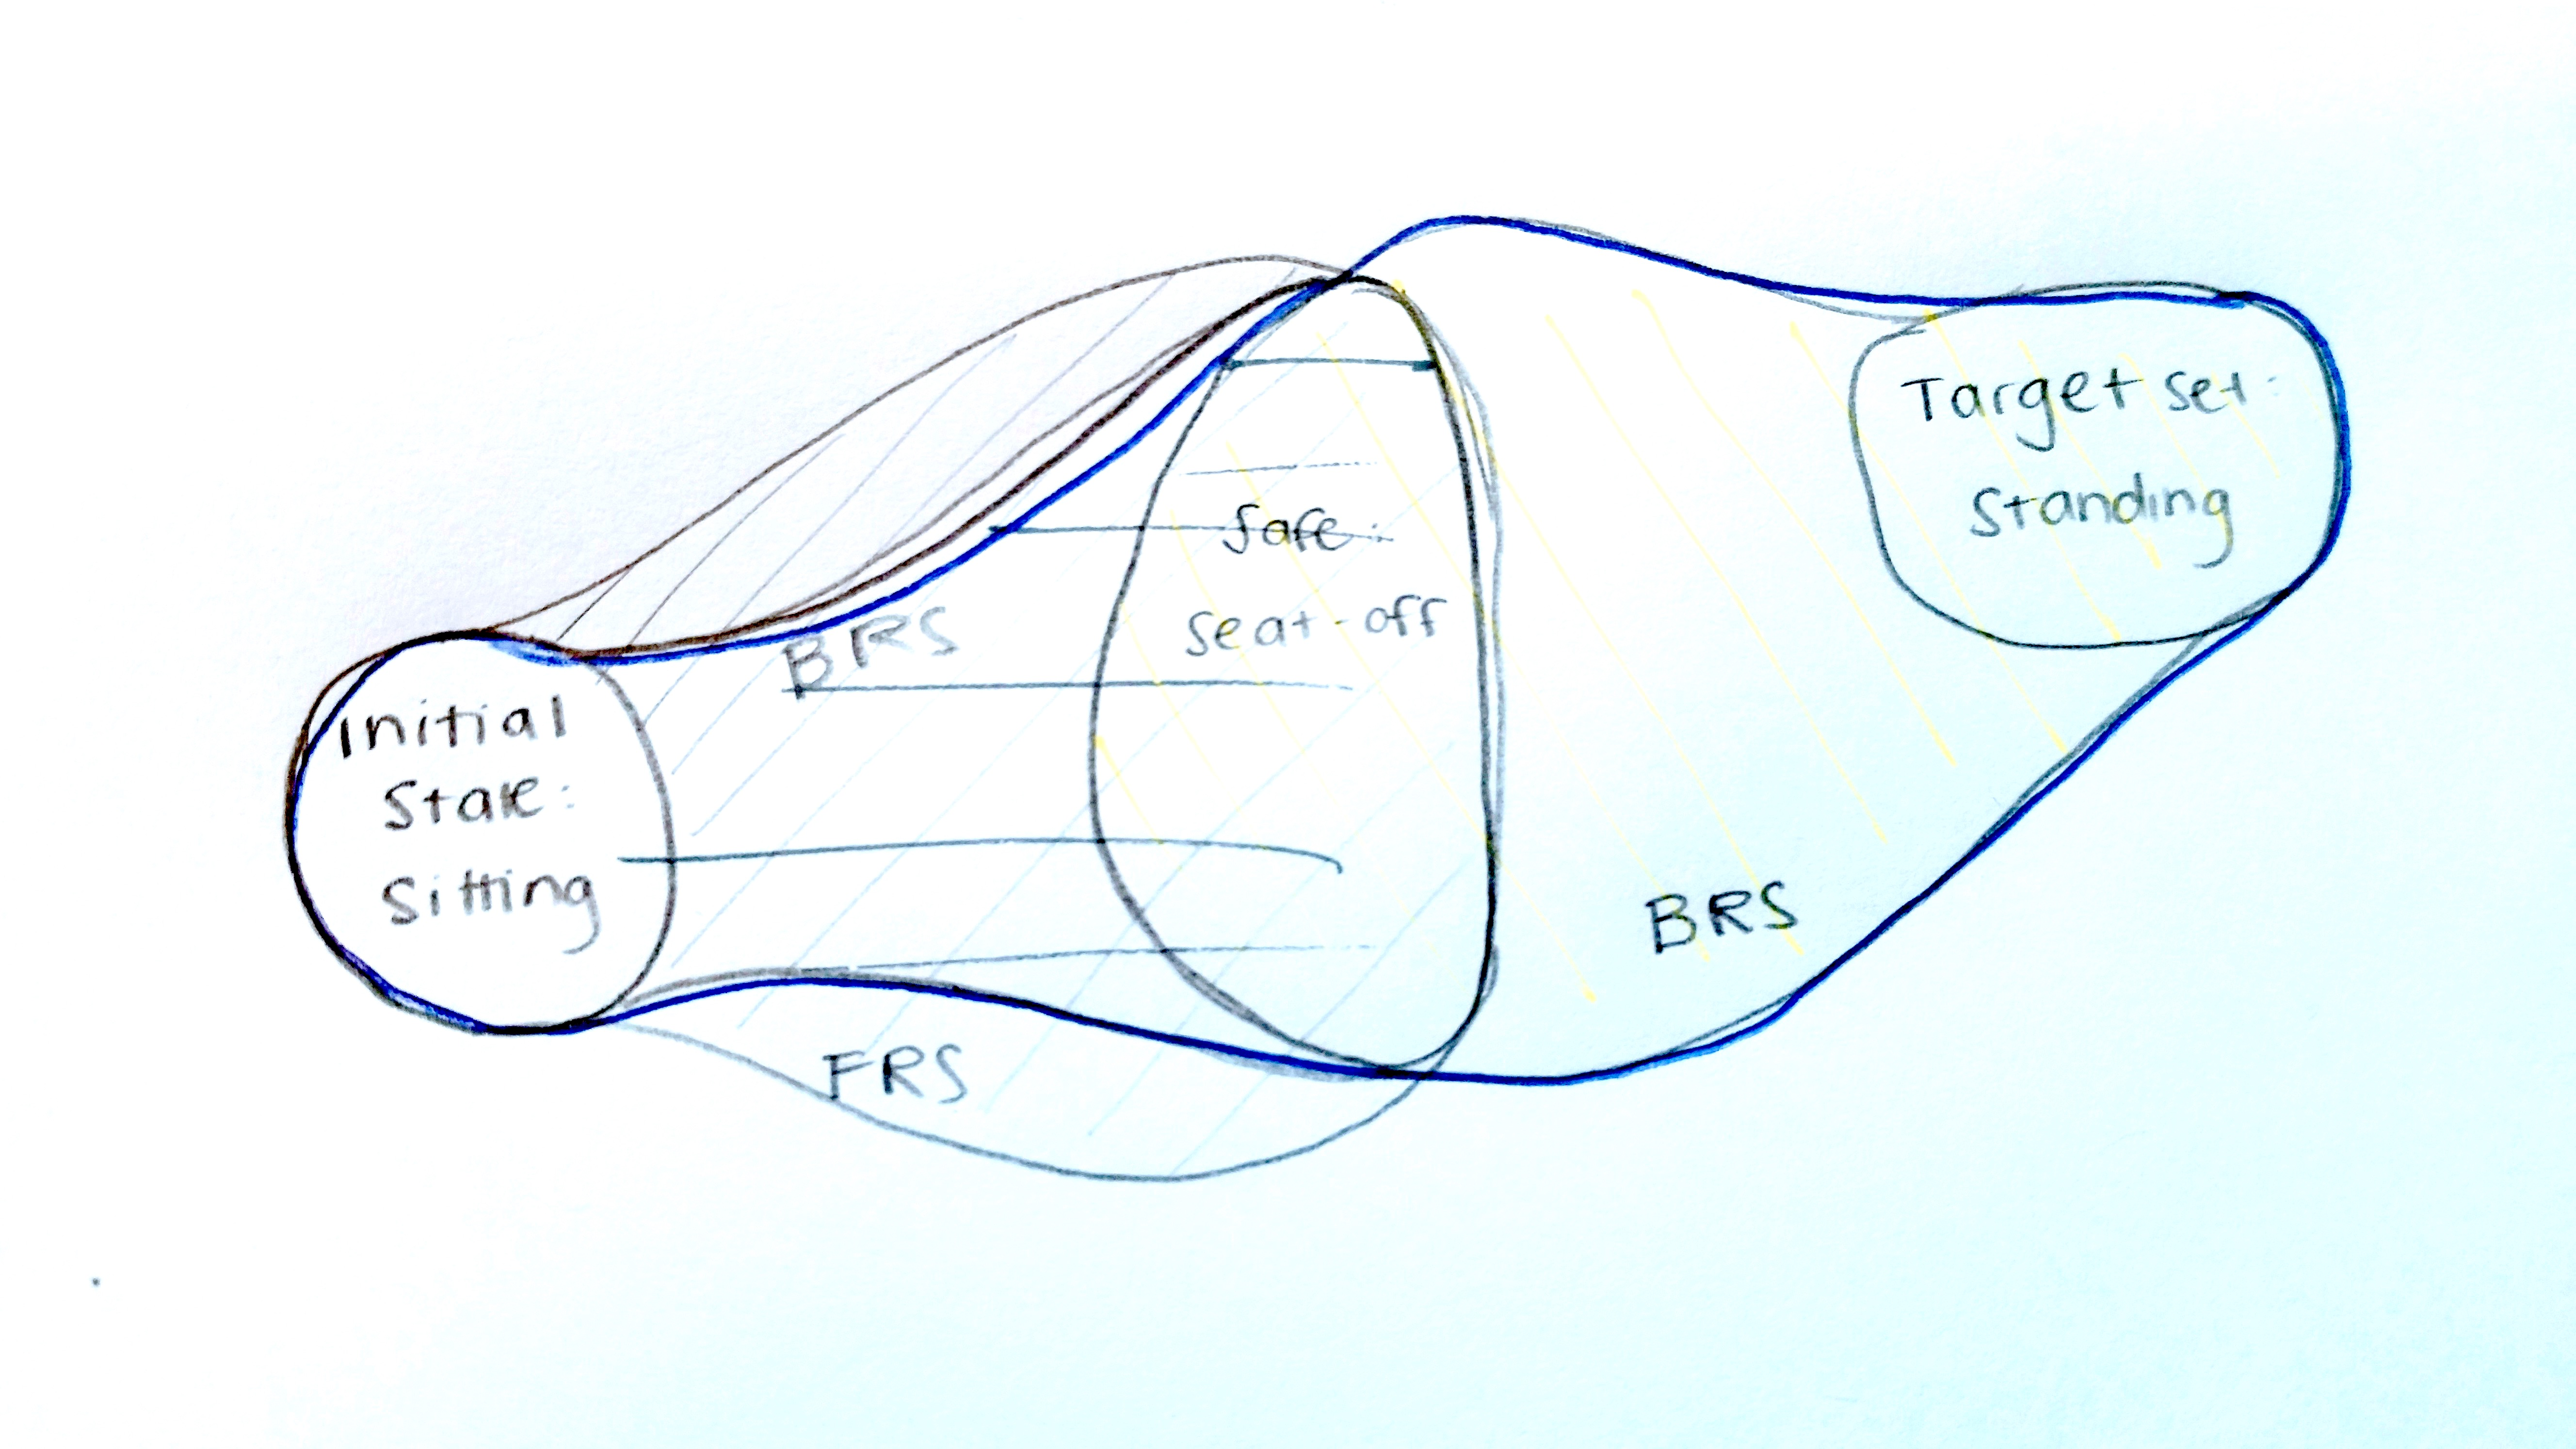
\includegraphics[width=3.5in]{figures/reachableSets.jpg}
	\caption{Reachable sets for STS motion.}
	\label{fig:hybrid}
\end{figure}

[Basic explanation of how HJ reachability analysis works]

We specify initial and final conditions on the states. The target set, representing the standing goal, is defined by a range of knee and hip angles near vertical with near-zero angular velocities. The initial seated condition is defined by a vertical HAT with zero-velocity. We compute a forwards reachable set, computing the set of states that be reached along trajectories which originate in the initial, seated position.

Separately, we compute a backwards reachable set, specifying conditions on the joint states which define the target set. The backwards reachable set represents the set of initial conditions of trajectories which enter the desired target set. In the case of sit-to-stand the backwards reachable set denotes the joint angles and velocities from which it is possible to reach a standing position. 

The intersection of the forwards and backwards reachable sets represent the states for which it is safe to transition between the seated and rising modes. From this final state, we compute a backwards reachable set to determine the allowable mode 1 states.
\section{Results}
hopefully..

\subsection{Experimental Validation}
An initial validation of this analysis method was performed on a single subject under informed consent (UC Berkeley IRB:2015-07-7767). The subject performed the sit-to-stand action with their arms crossed in front of them. Five STS motions were performed for three methods: 1) No guidance, 2) fast dynamic-standing, and 3) stabilization standing. The PhaseSpace Impulse X2  active motion capture system was used to collect kinematic data at 480 Hz. 

The method described in \cite{matthew2016} was used to extract joint angles and angular velocities for each STS motion. Due to the absence of force-data, seat-off was determined from the angular velocity of the knee joint. 



\section{Discussion}

This analysis method permits individualization of the model to a specific person or group, allowing for changes in model parameters and constraints placed on kinematic parameters (maximum joint range of motion and velocity) and dynamic parameters (maximum joint torque). Tools exist to measure an individual's torque limits and range of motion. Likewise, given knowledge of the presentation of a pathology, the STS motion for this population may be analyzed.
\subsection{Application to Coaching STS}
The intersection of the backwards reachable set from the standing target and the forward reachable set represent the set of states for which it is safe to leave the seat. Interpretation of this region can guide seat-off strategy, guiding an individual's trunk forward rotation and velocity prior to seat-off. 

This method may also be used to investigate the effects of other parameters which have been experimentally studied such as chair height \cite{schenkman1996}and initial footcite{khemlani1999}.

\section{Conclusion}
\subsection{Future Work}
Limitations....the current model implementation makes several assumptions and simplifications in the model. 

This framework allows for the inclusion of further constraints on the definition of safety.

\addtolength{\textheight}{-12cm}   % This command serves to balance the column lengths
                                  % on the last page of the document manually. It shortens
                                  % the textheight of the last page by a suitable amount.
                                  % This command does not take effect until the next page
                                  % so it should come on the page before the last. Make
                                  % sure that you do not shorten the textheight too much.

%%%%%%%%%%%%%%%%%%%%%%%%%%%%%%%%%%%%%%%%%%%%%%%%%%%%%%%%%%%%%%%%%%%%%%%%%%%%%%%%



%%%%%%%%%%%%%%%%%%%%%%%%%%%%%%%%%%%%%%%%%%%%%%%%%%%%%%%%%%%%%%%%%%%%%%%%%%%%%%%%



%%%%%%%%%%%%%%%%%%%%%%%%%%%%%%%%%%%%%%%%%%%%%%%%%%%%%%%%%%%%%%%%%%%%%%%%%%%%%%%%
%\section*{APPENDIX}
%
%Appendixes should appear before the acknowledgment.
%
%\section*{ACKNOWLEDGMENT}
%{roberts1996}
%The preferred spelling of the word �acknowledgment� in America is without an �e� after the �g�. Avoid the stilted expression, �One of us (R. B. G.) thanks . . .�  Instead, try �R. B. G. thanks�. Put sponsor acknowledgments in the unnumbered footnote on the first page.

%%%%%%%%%%%%%%%%%%%%%%%%%%%%%%%%%%%%%%%%%%%%%%%%%%%%%%%%%%%%%%%%%%%%%%%%%%%%%%%%

\bibliographystyle{IEEEtran} 
\bibliography{IEEEabrv,embc2017}


\end{document}
